






% =========----------	[ Space left here for distraction free mode] ----------==========%










\section{Post-Processing and Workflow Set Up} % Think of a better heading

	Once the recording at Abbey Road Studios was complete, the recording session was assessed using 5.1 surround sound system with a PC running ProTools 12 in the media suit at the University of York. In a normal audio editing situation the best bits of every take could be split and merged together. However as this would cause discontinuity in the video and the audio, coupled with the impracticality imposed by the abundance of audio tracks, a single take must be used. It was decided that take eight of 'Close Your Eyes' would be used as the track for testing. This take was exported and condensed into a smaller project where each track was exported as a WAV file ready to be imported into Reaper for Ambisonic processing.

% Once each audio track had been previewed, the next objective was to decide on the best take recorded during the session. Each take contained minor instrumental issues such as wrong notes and timing issues.

	\subsection{Video Post-Production}
		Before the audio could be mixed within an Ambisonic framework, the 360\textdegree~videos needed to be produced. This was to ensure that the sound sources were accurately aligned with the visual in the VR environment, i.e the audio of the lead vocals needed to sound as though they were coming from the lead vocals. As two different 360\textdegree cameras were used during recording, two different methods of spherical video production were used.

			\subsubsection{Video Stitching and Editing}

				\paragraph{Position A - 360\textdegree~perspective GoPro Omni}
					The GoPro Omni rig comes paired with a software suite including Omni Importer that can be used for easily importing 6 individual video files that can then be stitched together and edited to create a spherical video ready for use in a VR workflow using Kolor's AutoPano Video software. The videos files from the six GoPro cameras for take eight were imported using the Omni Importer software and stitched together in AutoPano Video. With time and experience it is possible to optimise the video stitching process to prevent the 'ghosting' effect in which subjects/objects placed too close to the GoPro Omni rig are distorted as they are split between two of the GoPro cameras and part of the subject/object is lost within a blind spot. It can be seen in the video that the guitarist have fallen victim to such an effect.\\

					Once stitched together the video was exported as an mp4 file and imported into Adobe Premiere Pro \cite{AdobePremiere} for further editing. The colour balance was adjusted to add some vibrancy to the visuals, before a title was added at the beginning of the video. Fades were also applied at the beginning and end of the video to stop the video starting and ending abruptly. The editing process in Adobe Premiere was simple but necessary to produce a video suitable for use in the VR experience and listening tests.

				\paragraph{Position B - 180\textdegree~ perspective Samsung 360}
					Videos shot using the Samsung 360 camera can be stitched and processed using Samsungs dedicated software 'Gear 360 Action Developer'\cite{actiondev}. As the camera only uses two fish eye lenses it is not possible to adjust where the software stitches the two videos together meaning that any ghosting effect that occurs can not be removed. As the Samsung 360 was placed further away from the musicians and the front facing lens was directed towards the entire ensemble, ghosting did not affect any subjects of interest. Once the video was stitched the same post-processing in Adobe Premiere was applied to the video.\\
			
			\subsubsection{Video Playback and Head-Tracking}
				 Kolor's GoPro VR Player \cite{GoProVR} can be used to open and preview 360 videos with built in head-mounted display (HMD) support allowing the video to be navigated using either the HMD's motion sensors or by clicking on the video and dragging. In the case of this project an Oculus Development Kit 2 (DK2) \cite{OculusDK2} headset was utilised. Using an external piece of software it is possible to send the head-tracking data from GoPro VR Player to Reaper to synchronise the soundfield rotation required for head movement. This is explained in section ~\ref{avsync}.


		\subsection{Audio Post-Production}
			
			\subsubsection{Creating a Higher-Order Ambisonics Template in Reaper}

				Reaper \cite{Reaper} is (at the time of writing) currently the only DAW that allows for up to 64 channels per track making it perfect for Higher Order Ambisonic (HOA) production. A Reaper template utilising a 36 channel bus for each of the microphone arrays was produced, allowing the microphone arrays to be encoded up to Fifth-Order Ambisonics. Each of the 36 channel buses for each of the microphones arrays were then routed to a 36 channel track containing a sound field rotator and Fifth-Order binaural decoder. \\
				
				The Eigenmike was imported and processed on its own 36 channel track and routed to a sound field rotator and 3\su{rd} decoder. As the Eigenmike was placed on its side during the recording session, the orientation was corrected by applying an additional sound field rotation.
				The B-Format recordings produced by the Soundfield ST450 MKII microphones created four tracks for each of the W, X, Y and Z information channels. The separate W, X, Y and Z channels were assigned to a four channel 'parent' track in Reaper. The Soundfield ST450's also required their own 4 channel First-Order Ambisonic tracks and decoders.\\

				Once the template was produced, the raw audio files were imported and grouped into the appropriate microphone groups. The following sections describe the processing of the raw audio files to produce a Fifth-Order head-tracking binaural mix. \\

			\subsubsection{Treatment and Ambisonic Encoding}
				Before anything was encoded into an Ambisonic format, Reaper 'ReaEQ' equalisation plugins were applied to each of the microphone tracks. It is important to EQ the tracks before Ambisonic encoding to prevent spherical harmonic distortion. In some instances where the microphones were placed close to the instruments, subtle filtering was applied such as a 6db reduction below 110Hz on the drum kit to reduce the overpowering bass drum in an attempt to increase the clarity of the mix. Individual microphone channels within an array were treated with the same equalisation to provide consistency for the listening tests. The spot microphones were treated by Mirek Stiles from Abbey Road Studio before being imported into the Reaper project. This was to ensure that the spot microphone recordings were of good tonal quality as a standard mix should be. \\

				Inserted in the FX chain next was a Fifth-Order AmbiX encoder. The AmbiX encoders use the ambiX Ambisonic format, with the Ambisonic Channel Number (ACN) ordering and SN3D normalisation conventions \cite{AmbixFORMAT}. The AmbiX encoder plug-ins provide a graphical interface from which one can position mono or stereo sound sources to specific azimuth and elevation angles around the VR environment, shown in figure~\ref{ambixEncode}.\\

				% Spot mics
				The spot microphones were duplicated and split into two groups. The first group was used to encode the spot microphones relative to the video from viewing position A and the second for viewing position B. This was done by opening the video in GoPro VR Player and setting the view to the reference 0\textdegree~position, in this case the centre of the drum kit. The individual spot microphones were then placed in the 3-dimensional space using the ambiX encoder plug-ins and using the Oculus DK2 as a visual reference. A B-Format impulse response of St Albans Cathedral \cite{OpenAir} was obtained from the OpenAir online impulse response library to create a convolution reverb effect on the lead and backing vocals. Using the AmbiX MCFX Convolver4 plug-in \cite{AmbixPLUGINS}, \cite{AmbixDOWNLOAD} inserted onto 4-channel auxiliary track, it was possible to achieve a 3-D reverb effect that suited the VR experience better than a standard mono or stereo reverb effect. The vocal tracks could then be sent individually to the B-Format reverb bus to achieve the required wet/dry ratio.

				% Microphone Arrays
				Each microphone array was encoded in the same way that they should naturally be listened to. For example, the OCT surround channels were encoded in the same position that the speakers are designed to be placed as described in section~\ref{sec:OCT9}. For other microphones arrays that are not designed to be fed straight to a specific speaker layout, each microphone channel was encoded into a position relative to the listener as the microphones were placed in the room.

				% PCMA
				The left and right pair of coincident microphones for the PCMA were routed through a stereo bus so that the microphone width can be adjusted using pan pots. The left and right buses were panned at 30\% and -30\% respectively creating a pair of virtual microphones that were angled at 70.5\textdegree{} from the centre position.

				\begin{figure}[h]
				\begin{center}
					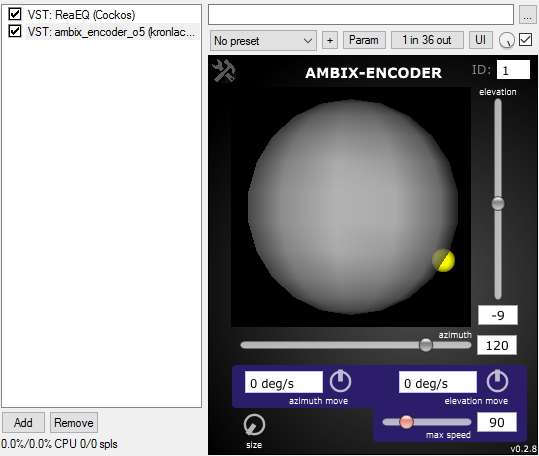
\includegraphics[width = \linewidth]{images/other/ambix.png}
					\caption{Screenshot of the Fifth-Order AmbiX encoder for a mono sound source (Kick Drum)}
					\label{ambixEncode}
				\end{center}
				\end{figure}

				% ST450
				For the raw SoundField ST450 recordings it was necessary to convert the Soundfield's B-Format recordings from the Furse-Malham format to the ambiX format using the AmbiX Converter plug-in \cite{AmbixPLUGINS}, \cite{AmbixDOWNLOAD}, which corrected the channel sequence and normalisation before the decoding stage. Apart from the format conversion, no other Ambisonic encoding was required as the Soundfield ST450 MKII microphone captured the full spherical soundfield with sound sources already in the correct locations. \\

				% Eigen
				Before importing into the reaper project, the Eigenmike recording was encoded into Third-Order Ambisonics using the EigenUnits plug-in by mh acoustics \cite{eigen}. This then meant the 36 channel 3\su{rd} order Eigenmike track could be imported into the Reaper project without the need to encode the track in real time. As the Eigenmike was mounted on its side during the recording session, the soundfield had to be rotated by -90\textdegree{} in the elevation plane to compensate for this positioning using an AmbiX Third-Order Rotator \cite{AmbixPLUGINS}.

			\subsubsection{Binaural Decoding}

				Each of the microphone array channels and spot mics were routed to a final mixing bus used for 5\su{th} order decoding. The Egienmike and Soundfield microphones were sent to a 3\su{rd} order and 1\su{st} order mix bus respectively. An ambiX Binaural Decoder plugin was inserted onto each of the mix buses. The plug-in requires a configuration files that contains information regarding where the HRTF data set to use is stored, the virtual loudspeaker layout that should be used and provides a decode matrix to multiple the signal vector by \cite{Girafe}. Configuration files for the following Ambisonic orders and speaker layouts were taken from the SADIE database \cite{SADIE}:

				\begin{center}
				%\resizebox{0.45\textwidth}{!}
				\end{center}


				As Google have recently adopted the KU100 measurements from the SADIE database to use in their YouTube360 \cite{youtube360} online platform, the same HRTF data set was used in the binaural decoding process. The HRTF set first needed to be converted from 44.1kHz/16-bit as downloaded from the SADIE database to 48kHz/24-bit to match the settings of the Reaper project using the r8brain V1.9 \cite{r8brain} application.

		\subsection{Audio Visual Synchronisation}\label{avsync}

			When turning your head in the real world, sound sources remain static in 3D space and your perspective of the world is rotated both visually and sonically. When listening to a binaural decode over headphones however, when you turn your head the headphones and the audio being played through them stay in place on your head. If something was encoded you sound like it was coming from your right, it would sound like it was coming from your right no matter where you turned your head. To create a truly immersive audio visual environment the sound field must be rotated as the visuals are. This can be achieved by using a sound field rotation plug-in and feeding it real time rotation data. 

			SpookSyncVR \cite{SpookSync} is built in Max MSP as a stand-alone application that allows data exchange between GoPro VR Player and Reaper using Open Sound Control (OSC). Using SpookSyncVR it is possible to gather the X (yaw) and Y (pitch) rotation data from the headset and transfer the information to Reaper so that the sound field can be rotated accordingly. For this an Ambix Rotator plug-in was inserted into each of the three decoder tracks just before the binaural decoding plug-in for which the yaw and pitch data from GoPro VR Player were assigned to control the values of the yaw and pitch data of the rotator plug-ins. By designating the GoPro VR Player as the 'master' and Reaper as the 'slave' it was possible to synchronise, play and stop the audio and video together. 
	
		
